Um den betroffenen Nutzer zur Zahlung der Lösegeldsumme zu überreden, spielen den Angreifern mehrere Faktoren in die Hände. Diese sind eher unbewusst eingebaut, da sich die Angreifer nicht noch zusätzlich beispielsweise Psychologen in ihr Team holen, um durch vermehrte psychologische Faktoren möglichst viel Gewinn zu erzielen. Im Bereich Internationalisierung\cite{faktoren:l18n}, Usability und grafische Aufbereitung\cite{faktoren:grafik}\cite{evolution} kann jedoch davon ausgegangen werden, dass hier auf professionelle Hilfe zurückgegriffen wurde.

\subsection{Psychologische Aspekte}

Da Locker- und Crypto-Ransomware verschiedene Punkte der menschlichen Psyche müssen diese gesondert behandelt werden:

Die Locker-Ransomware ``Lockdroid.G''\ref{fig:lockdroid}, die Android-Smartphones angreift, nutzt etwa Täuschung. Kognitive Mechanismen nutzen gerne Abkürzungen, um so die gedankliche Effizienz zu steigern. Dies ist der Grund dafür, dass Täuschungen wie etwa das Abbilden von Strafverfolgungsbehörden-Logos dazu führt, dass Menschen die Legitimität der Meldung nicht anzweifeln. 

\begin{wrapfigure}{r}{0.3\textwidth}
  \begin{center}
    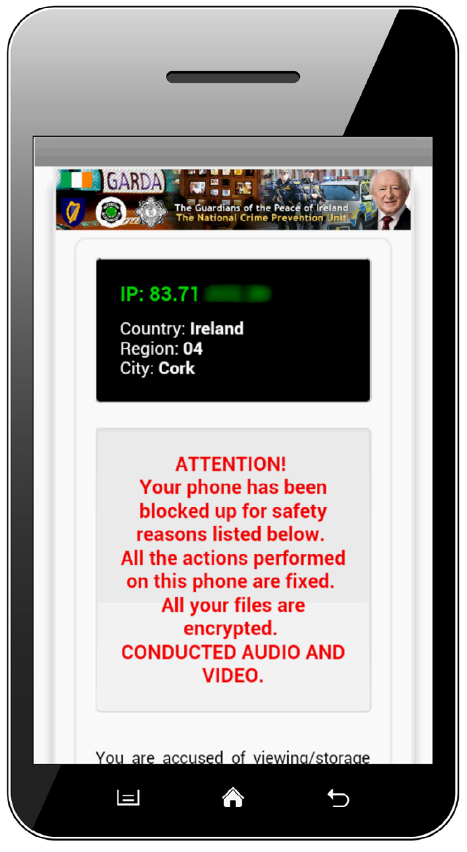
\includegraphics[width=0.48\textwidth]{img/android_locker.png}
  \end{center}
  \caption{Locker am Beispiel ``Lockdroid.G''\cite{evolution}}
  \label{fig:lockdroid}
\end{wrapfigure}

Das Elaboration Likelihood Model geht davon aus, dass es 2 Wege zur Überzeugung gibt. Überzeugung durch die zentrale Verarbeitung der Mitteilung beschreibt die Abwägung und Qualität der Argumente. Hierbei wird also mit wohl überlegten Argumenten gearbeitet, um das Opfer zur Zahlung des Lösegelds zu bewegen. Im Falle von ``Lockdroid.G'' wäre das etwa die Tatsache, dass die Polizei das Smartphone ``aus Gründen der Sicherheit'' sperrt.\\
Die periphere Verarbeitung der Mitteilung beschreibt dagegen eher konditionierte Verhaltensweisen. Es wird davon ausgegangen, dass negativ oder positiv konnotierte Stichwörter zum Ergebnis führen. Als Beispiele hierfür kann z.B. das Logo der Polizei dienen oder auch die Anzeige des Landes, IP-Adresse und Stadt, die beim Opfer zur Angst führen, dass er etwas Illegales getan habe. \\

Wird noch angezeigt, dass der Nutzer illegal Dateien wie Musik oder Filme herunter geladen habe, führt dies dazu, dass er aus Angst vor sozialer Stigmatisierung nicht bei Bekannten oder der Polizei um Hilfe bittet.\\

Während Locker-Ransomware eher mit den psychologischen Faktoren innerhalb der Nachricht arbeitet, benutzt Crypto-Ransomware die Empfindungen den verschlüsselten Daten gegenüber und welchen Schaden das Opfer hätte, diese wertvollen Daten zu verlieren.\\

Zum einen enhalten viele Crypto-Ransomwares einen Countdown, nach dessen Ablauf die Daten endgültig verloren seien. Der Faktor Zeit wurde schon in Tests auf irrationale Entscheidungen hin untersucht. Zudem kann zum Countdown die Lösegeldforderung höher werden, je weiter die Zeit voran schreitet. Das setzt das Opfer so unter Druck, dass dieses bereitwillig bezahlt.\\
Das Ellsberg-Paradoxon der Entscheidungstheorie beschreibt das Verhalten von Menschen, die sich in einer Situation mit umgewissen Ausgang befinden. Wenn sie mit 2 Möglichkeiten konfrontiert sind, deren eine Möglichkeit einen Gewinn darstellt, dessen Wahrscheinlichkeit aber nicht abzusehen ist und der anderen Möglichkeit, dass sie etwas verlieren, aber dieser Verlust von der Wahrscheinlichkeit abzuschätzen ist, so nehmen Menschen eher den Verlust in Kauf.\\
Im Falle von Crypto-Ransomware haben die Menschen es mit 2 negativen Möglichkeiten zu tun: Einmal können sie nicht sicher sein, ob sie durch Bezahlung ihre Daten wieder erhalten. Auf der anderen Seite können sie noch weniger sicher sein, wieweit der Verlust ihrer Daten sie beeinflusst. Auch hier ist die Tendenz eher Richtung bezahlen und auf Wiedererhalt der Daten hoffen.

\begin{figure}[h!]
	\centering
	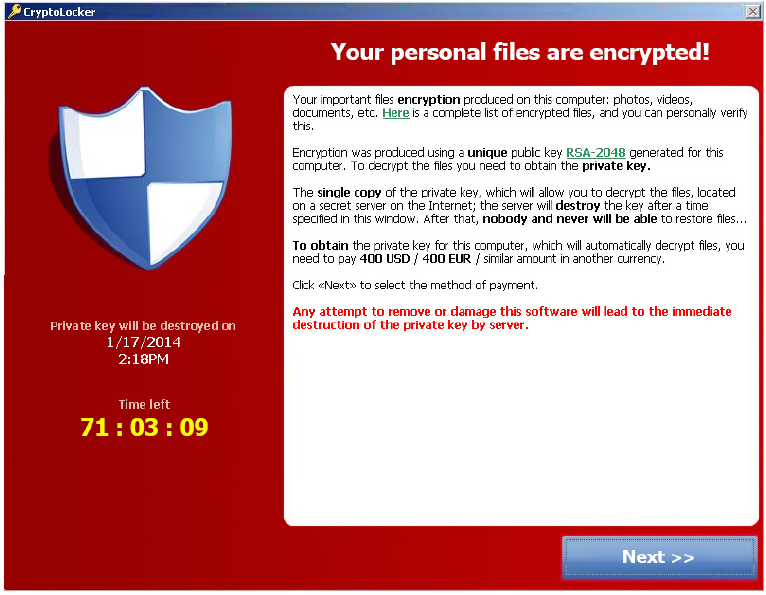
\includegraphics[width=\textwidth]{img/cryptolocker.png}
	\caption{Crypto-Ransomware am Beispiel ``Cryptolocker''\cite{evolution}}
	\label{fig:cryptolocker}
\end{figure}


\subsection{Preis und Bezahlsysteme}

Bereits die AIDS Ransomware hatte als Lösegeldsumme circa 300 \$ (Inflation eingerechnet), was dem Preis aktueller Ransomware entspricht\cite{evolution}.\\ 
Die durchschnittlichen Einkommen der unterschiedlichen Länder finden sogar Einzug in Ransomware: Um das Opfer zur Zahlung zu bewegen, darf sich die Lösegeldforderung nicht auf einem Level befinden, welches die Einkommensgrenze überschreitet. So wird in Ländern wie beispielsweise Indien oder Rumänien etwa ein anderer Betrag gefordert als in den USA und Deutschland. Technisch wird dies dadurch gelöst, dass sich ein infizierter Rechner bei dem Command-and-Control-Server der Angreifer meldet und dieser dadurch anhand der IP-Adresse eine grobe Zuordnung nach Ländern treffen kann.\\

Eine weitere Anpassung beim Preis wird bei der Unterscheidung zwischen Privatperson und Firma getätigt: Wird festgestellt, dass eine Firma betroffen ist, so werden einige Tausend Dollar verlangt, um die Daten zurückzuerhalten. Sicherheitsexperten haben heraus gefunden, dass der ideale Punkt, den Firmen noch bereit sind zu zahlen, und bei dem die Polizei noch keine Ermittlungen beginnt, bei 10.000 \$ liegt\cite{sweetspot}.\\

Um den Strafverfolgungsbehörden zu entgehen, ist es für die Ransomware-Community notwendig, anonym bezahlt zu werden, da sich so keine Spuren nachverfolgen lassen. War dies zur Zeiten von AIDS noch ein anonymes Postfach in Panama, so hat sich das im Digitalzeitalter geändert. Anfangs wurde noch der Anruf einer kostenpflichtigen Nummer oder die Bezahlung mit Bezahlgutscheinen wie Pasafecard oder CashU präferiert, inzwischen ist der Fokus bei Kryptowährungen wie Bitcoin. Diese ermöglichen es anonym zu bleiben und den Geldfluss nicht verfolgen zu können.\\

Interessant ist auch, dass je nach Ransomware-Art andere Bezahlsysteme zum Tragen kommen. Während durch Lockern der Rechner gesperrt ist, können etwa keine Bitcoins online gekauft werden, um mit diesen der Lösegeldforderung nachzukommen. In diesem Fall wird dann auf Bezahlgutscheine zurück gegriffen, die es einfach und schnell an vielen Tankstellen und Supermärkten zu kaufen gibt. Dagegen ist bei Crypto-Ransomware der Rechner noch bedienbar, also können noch Bitcoins erworben werden. Je nach Ransomware wird sogar ein Video als Anleitung dazu gezeigt.

\subsection{``Probepackung''}

Um dem Opfer zu demonstrieren, dass es die verschlüsselten Dateien wieder entschlüsselt bekommt, sollte es den Betrag bezahlen, bietet manche Ransomware an, dass eine handvoll zufällig ausgewählte Dateien des Rechners entschlüsselt werden. Dies steigert das Vertrauen der Opfer und erhöht die Chancen einer Bezahlung.